\documentclass[11pt, a4paper]{jsarticle}
\usepackage{multicol}  % パッケージの追加
\usepackage[dvipdfmx]{graphicx}
\begin{document}
%=============================================================
%=============================================================
\section{Holography - two-beam transmission hologram}
\subsection{Two-beam transmission holograms}
\subsubsection{Purpose}
前回の二光干渉による回折格子の製作の原理を用いてホログラムを作る.
ホログラムの原理を理解する.
\subsubsection{Contents}
以下のように光学系を製作する.

\begin{figure}[htbp]
 \begin{center}
  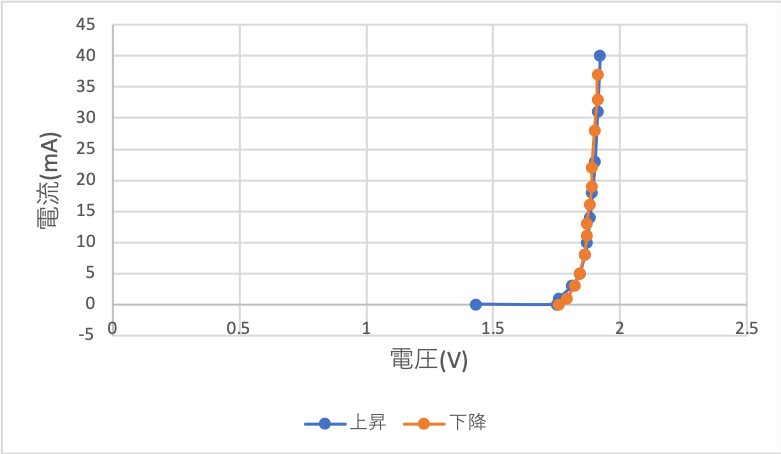
\includegraphics[width=100mm]{fig23.png}
 \end{center}
 \caption{二光干渉によるホログラムの実験}
 \label{fig:23}
\end{figure}

まず今回は5\%のビームスプリッターを使用した.また分けたそれぞれの光をL1,L2のレンズによって拡大した.L1によって拡大された光を物体にあて反射光がプレートホルダーに届くように調節した.この時Objectとして白鳥のモデルを使用した.
また前回から基本的に実験機材を動かしていないため二つの光路差は0となっておりコヒーレント長を上回らないことを確認した.
またプレートホルダー上において参照光の強度がと物体光の強度が2から3倍となるように計測器を用いて調節した.

この時参照光強度は0.55μW,物体光強度は0.20μWであった.
以上結果よりフィルムプレートに露光する時間を計算する.
ホログラムを作るのに最適な露光時間は$90[\mu J/cm^2]$であるので計測器の面積が$16\pi [mm^2]$であることに注意すると露光時間は60.32[s]と計算できる.

露光が終わったら次は現像作業を行う.
現像は以下のような手順で行なった.

\begin{table}[htb]
  \begin{center}
    \caption{現像の手順}
    \begin{tabular}{|l|l|l|l|} \hline
       項目&&内容&処理時間\\ \hline
       現像&\begin{tabular}{c}現像液\\コピナール\end{tabular}&ホログラム乾板を浸し連続撹拌する&6分\\ \hline
       水洗い&水&水ですすぐ&2分\\ \hline
       定着&\begin{tabular}{c}定着液\\スーパーフィジフィックス\end{tabular}&ホログラム乾板を浸し連続撹拌する&5分\\ \hline
       予備水洗い&水&水ですすぐ&2分\\ \hline
       水洗促進浴&\begin{tabular}{c}水洗促進剤\\フジQW\end{tabular}&浸しながら撹拌する&1分\\ \hline
       水洗い&水&水ですすぐ&2分\\ \hline
       脱水&\begin{tabular}{c}仕上げ剤\\ドライウェル\end{tabular}&浸しながら撹拌する&1分\\ \hline
       乾燥&ドライヤー&ドライヤーの弱冷風を当てる&乾くまで\\ \hline
    \end{tabular}
    \label{tab:1}
  \end{center}
\end{table}

現像後5\%ビームスプリッターを100\%ビームスプリッターに取り替え参照光を現像したフィルターにあてフィルター越しに干渉光を覗き込んでホログラムが作られているかを確認する.
\subsubsection{Result}
現像したフィルターに参照光を当て覗き込むと下の写真のような像が観察できた.
またこの像は写真などとは異なり三次元的に映し出されていた.

\begin{figure}[htbp]
 \begin{center}
  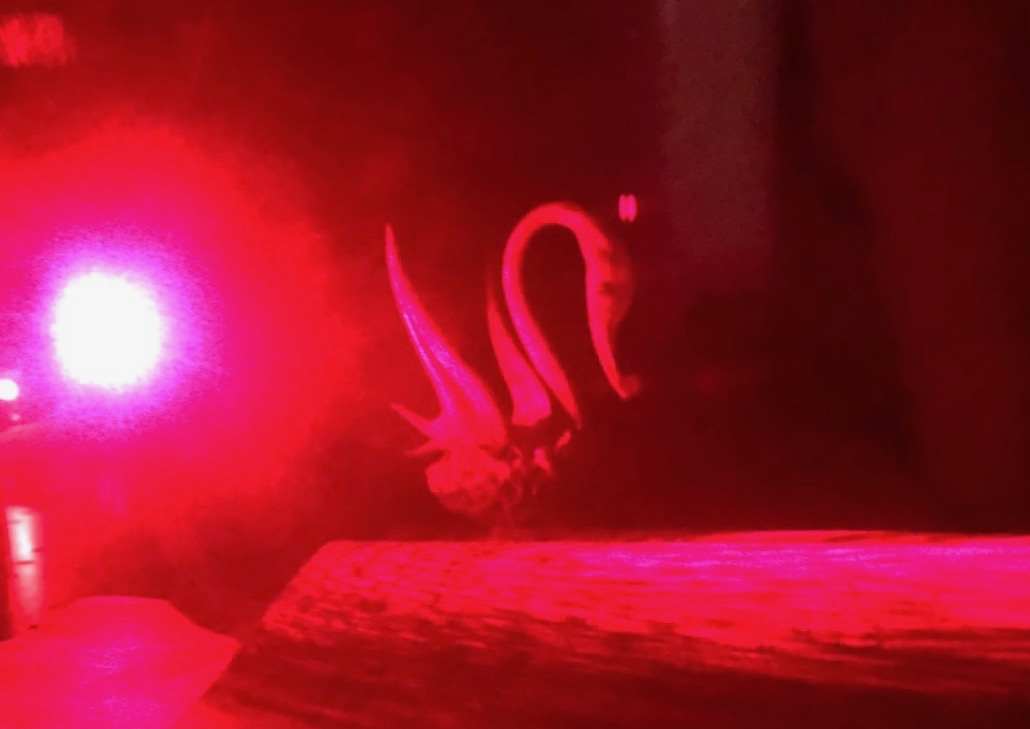
\includegraphics[width=100mm]{fig24.png}
 \end{center}
 \caption{白鳥のホログラム}
 \label{fig:24}
\end{figure}
\newpage
\subsubsection{Discussion}
まず,今回はコヒーレント長を上回らなっかたためにしっかりフィルター上にホログラムを作る回折格子が作られたと考えられる.
もし光路差がコヒーレンス長を上回ってしまった場合はフィルター上で干渉を起こすことができずに綺麗にホログラムが生成されないことが予測される.
そのため光路差を等しくする作業はこの実験において非常に重要な操作であったと考えられる.
また今回の実験で得られたフィルターが割れたとしてもその破片に同じように参照光を同じ角度で当てるとこのホログラムは再現されると予想される.
これはホログラムが再生されるためのフィルター上の回折格子の間隔は前回の実験から分かるように数μmのオーダーであるからである.
そのためある程度小さくプレートを割ったとしてもホログラムが再生されることが予想される.

また今回のホログラムの生成は原理としては実験5の二光干渉によってできた回折格子による干渉と同じである.
今回の場合は前回の実験と異なり白鳥のオブジェクトから反射された光と参照光によってプレート上に回折格子が作られた.
このプレートに参照光を照射した際に透過光の複素振幅が物体光に比例する光が再生されるためだと説明できる.
この現象は以下の式によって説明される.

まず光電場を$E(\vec{r},t) = A_0e^{i(\vec{k} \cdot \vec{r} - {\omega}t)} = \Psi e^{-i{\omega}t}$
ここで複素振幅$\Psi = A_0e^{i\phi}$ ($\phi = \vec{k} \cdot \vec{r}$)
とする.
するとまずプレート上では参照光と物体光が干渉を起こすのでプレート面での複素振幅$\Psi_H$は
\begin{eqnarray*}
  \Psi_H = \Psi_O + \Psi_R
\end{eqnarray*}
ここで$\Psi_O,\Psi_R$はそれぞれ物体光と参照光の複素振幅を表す.
したがってプレート上でのビーム光の強度$I_H$は
\begin{eqnarray*}
  I_H &=& (\Psi_O + \Psi_R)(\Psi_O + \Psi_R)^\ast \\
      &=&|\Psi_O|^2 + |\Psi_R|^2 + \Psi_R\Psi_O^\ast + \Psi_O\Psi_R^\ast
\end{eqnarray*}
プレート上の感光材がこの光強度$I_H$に比例した透過率変化を起こすはずなのでこのプレートに参照光のみを照射した際に生成される透過光複素振幅$\Psi_T$は比例定数Kを用いて
\begin{eqnarray*}
  I_H &=& K\Psi_R[|\Psi_O|^2 + |\Psi_R|^2 + \Psi_R\Psi_O^\ast + \Psi_O\Psi_R^\ast] \\
    &=& K[\Psi_R(|\Psi_O|^2 + |\Psi_R|^2) + \Psi_R^2\Psi_O^\ast + \Psi_O|\Psi_R|^2]
\end{eqnarray*}
この時第三項の複素振幅$\Psi_O|\Psi_R|^2$は物体光の強度に比例するため,参照光の透過光により物体光が再生されることが数式によっても示された.

% \end{multicols}
\begin{thebibliography}{99}
 \bibitem{光物理学} 櫛田孝司『光物理学』(共立出版,1983)
\end{thebibliography}

%==========================================================
%==========================================================
\end{document}
